\chapter{Materiales y métodos}
\thispagestyle{empty}

\section{Materiales}

\subsection{Modelos 3D}
%En este apartado se describe cómo se obtuvieron los conjuntos de datos 3D y las decisiones tomadas para elegir unos dataset frente a otros. Además, se explicará el subconjunto de casos elegidos para generar las fotografías faciales 2D.

Para este TFG, se llevó a cabo un análisis exhaustivo de las bases de datos disponibles de modelos 3D de personas. Tras la búsqueda, se utilizaron diversos conjuntos de datos públicos con el objetivo de crear un conjunto de datos unificado, realista y diverso. En este conjunto, se incluyeron tanto modelos faciales como modelos de cuerpo completo.

\subsubsection{Modelos faciales}
% Hablar de que se quiere mejorar el conjunto de datos usado en FacialSCDnet (Stirling)
% Modelos más realistas y diversos
Se han seleccionado los siguientes conjuntos de datos: HeadSpace \cite{60}, H3DS-net \cite{61} y DI4D\_UGR\_ANON \footnote{Conjunto de datos proporcionado por el tutor}.

El conjunto de datos de Headspace \cite{60} es un conjunto de imágenes en 3D de la cabeza humana, que consta de 1519 sujetos que llevan gorros de látex ajustados para reducir el efecto de los peinados. Las ventajas de este conjunto son que tienen muy buena resolución y además incluye metadatos útiles para seleccionar un subconjunto de datos adecuado.

\begin{figure}[h]
	\centering
	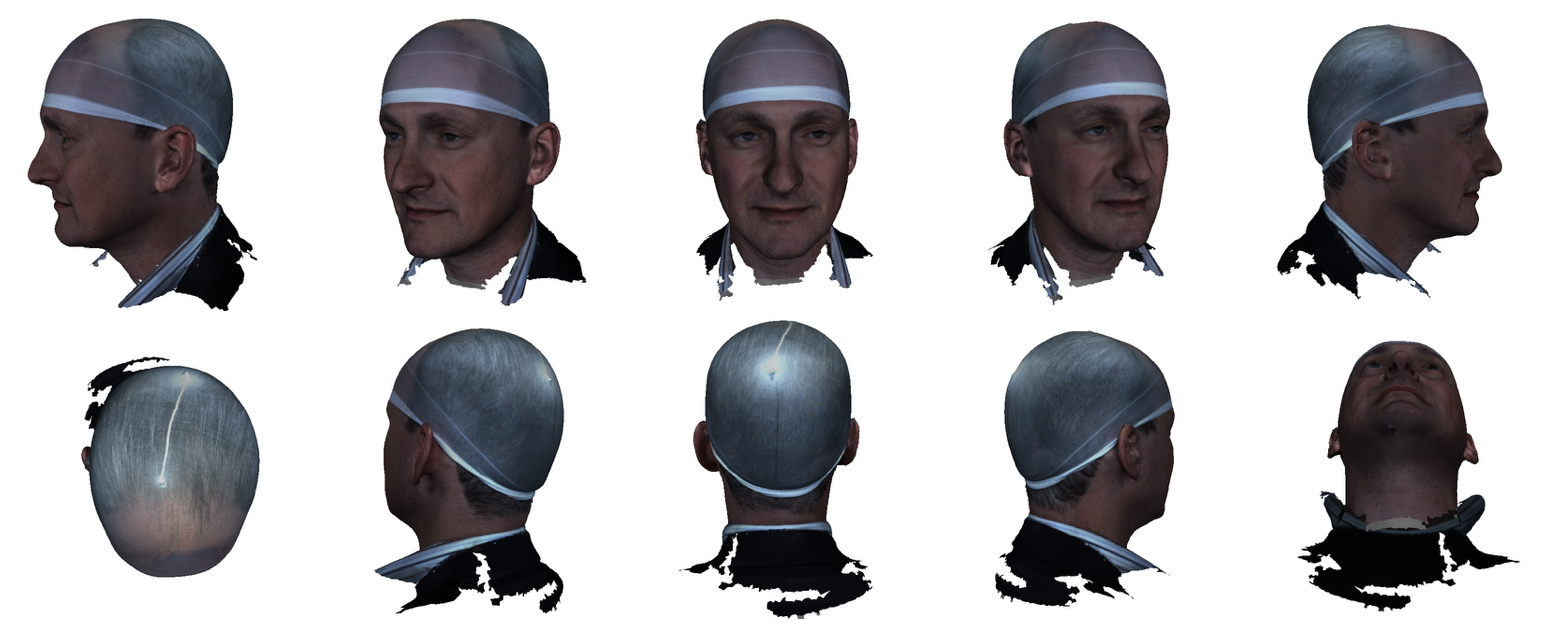
\includegraphics[scale=0.35]{imagenes/cap4/headspace.png}
	\caption{HeadSpace 3D}
	\label{fig1}
\end{figure}

H3DS-net \cite{61} contiene escaneos texturizados en 3D de la cabeza completa con una alta resolución. Este conjunto comprende un total de 23 modelos, todos ellos con los ojos cerrados, lo que añade una variabilidad adicional.

% Cambiar esta imagen y hacerla yo
\begin{figure}[h]
	\centering
	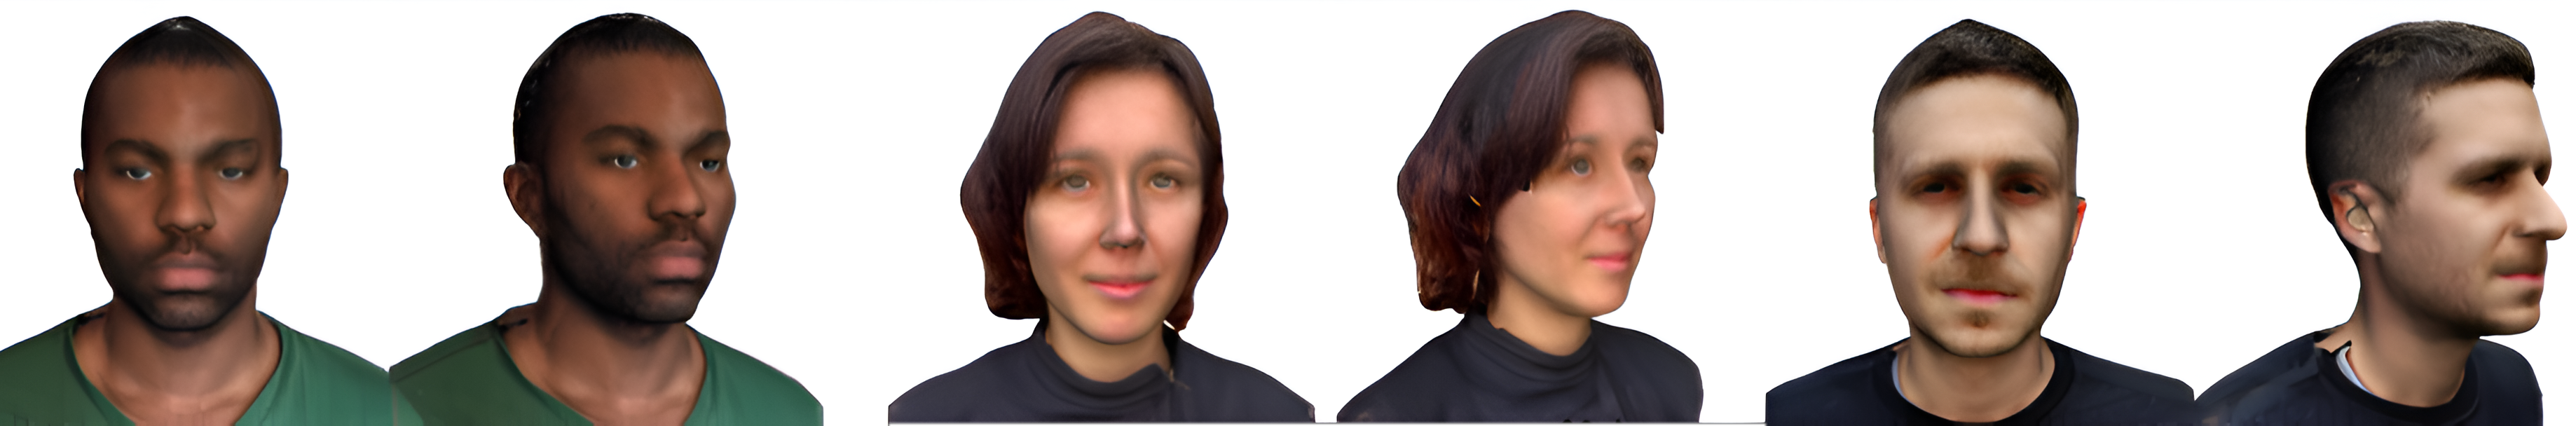
\includegraphics[scale=0.1]{imagenes/cap4/h3dsnet2.png}
	\caption{H3DS-net}
	\label{fig2}
\end{figure}

DI4D\_UGR\_ANON es un conjunto de datos creado por la Universidad de Granada...


% Incorporar fotos de cada 

Si bien se investigaron otros conjuntos de datos como FaceVerse \cite{64} o CASIA \footnote{http://biometrics.idealtest.org/}, estos fueron descartados debido a problemas como la baja calidad, formatos incompatibles y escalas no reales.

\subsubsection{Modelos de cuerpo entero}
Se han seleccionado los siguientes conjuntos de datos: HuMMan \cite{62}, People Snapshot \cite{63} y Render People \footnote{https://renderpeople.com/es/}

\begin{figure}[h]
	\centering
	\includegraphics[scale=0.4]{imagenes/cap4/humman2.png}
	\caption{HuMMan}
	\label{fig3}
\end{figure}

\begin{figure}[h]
	\centering
	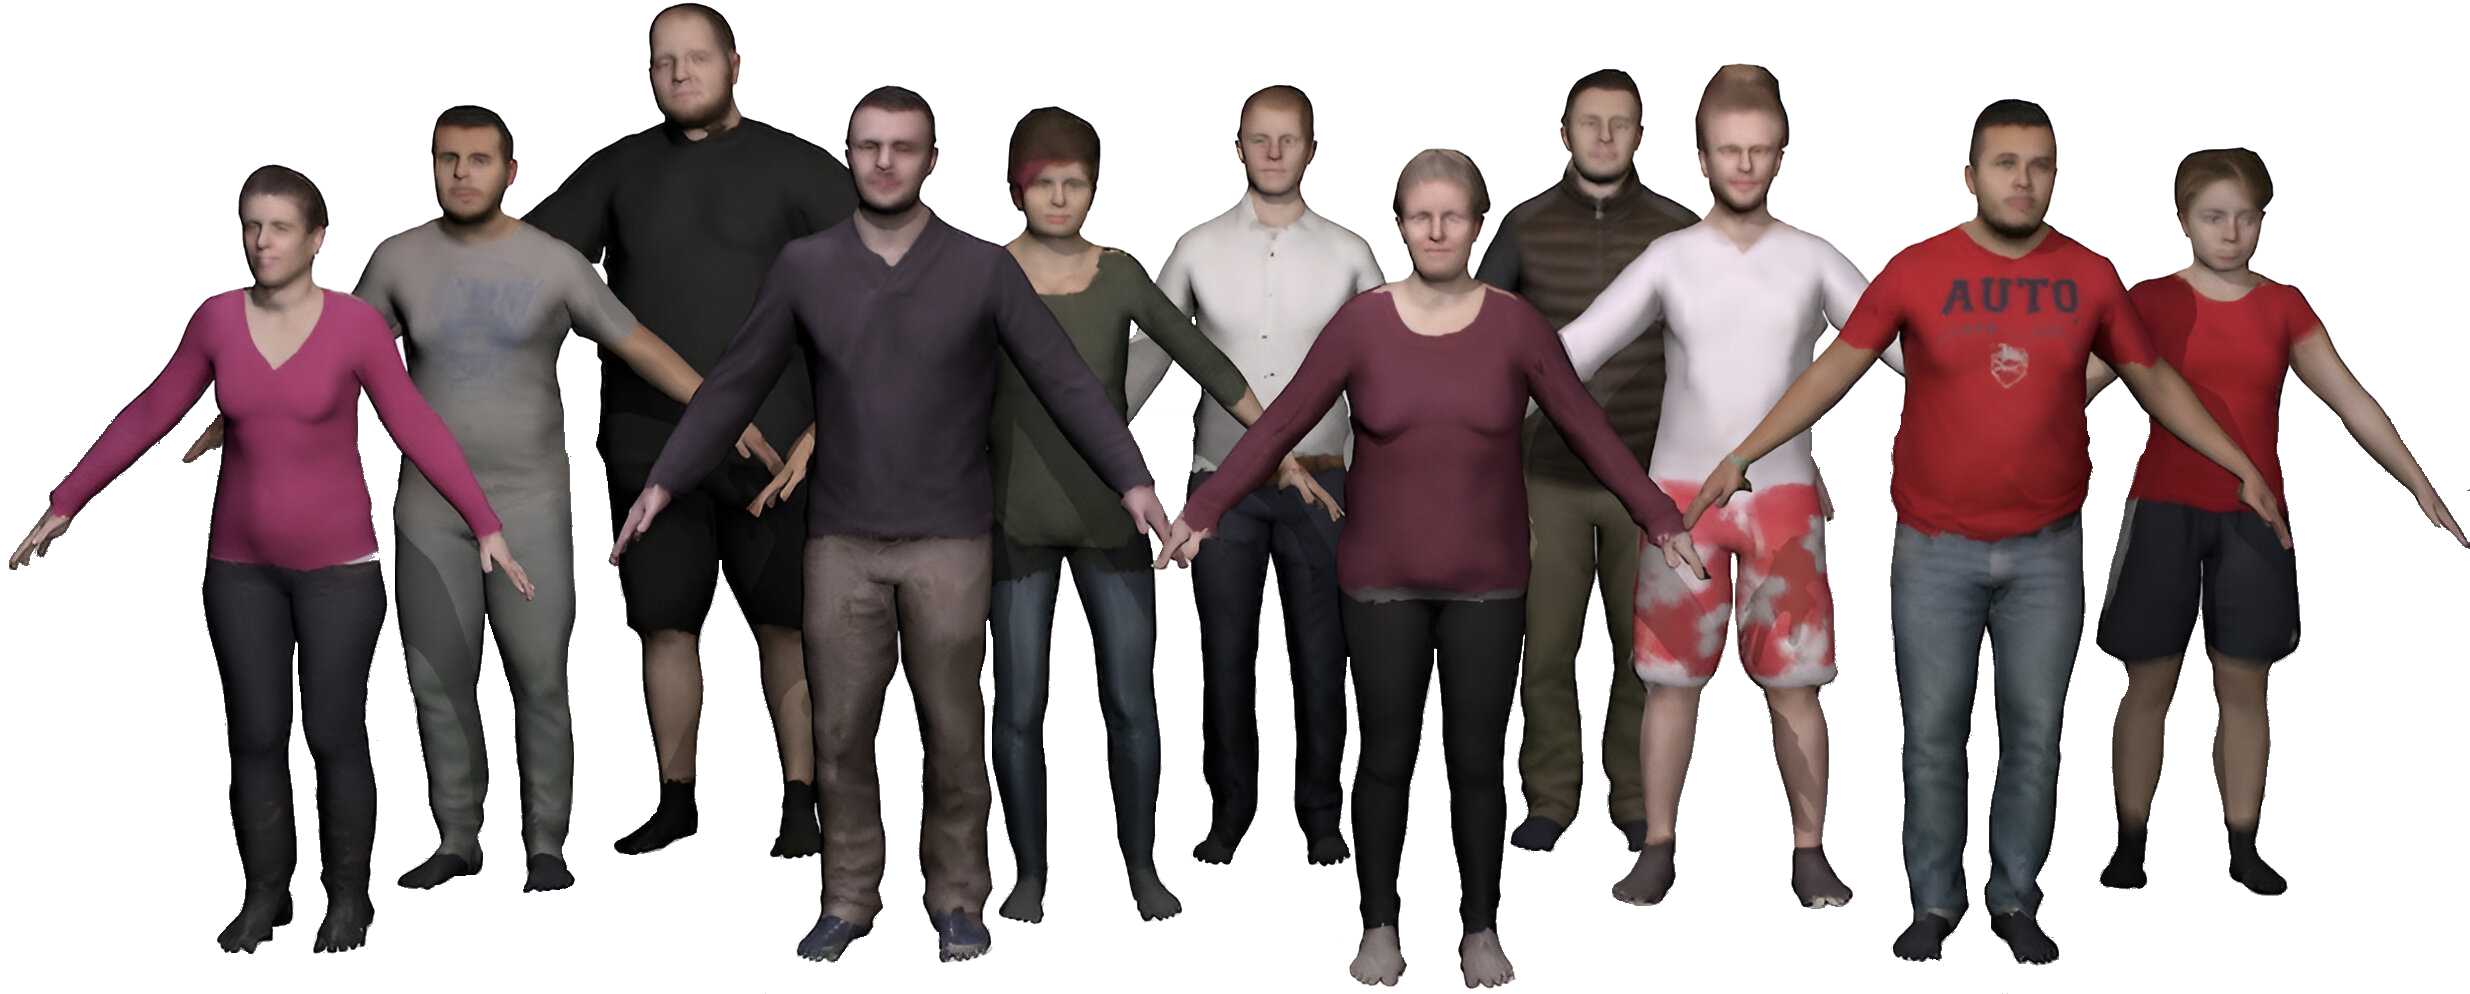
\includegraphics[scale=0.5]{imagenes/cap4/snapshot2.png}
	\caption{People Snapshot}
	\label{fig4}
\end{figure}

\begin{figure}[h]
	\centering
	\includegraphics[scale=0.04]{imagenes/cap4/renderpeople2.png}
	\caption{Render People}
	\label{fig5}
\end{figure}

\subsubsection{Selección del subconjunto de datos}

% Hablar de cuántos y de qué tipo de modelos hemos escogido

\subsection{Procesamiento del conjunto de datos}
En este apartado explicaremos la necesidad de alinear los modelos 3D para tener el origen a la altura de los ojos y así poder tener una referencia a la hora de generar imágenes 2D a distintas distancias. Se expondrán los métodos llevados a cabo para dicha finalidad (tanto alinear como generar las imágenes). Además, se explicará cómo se han cambiado los fondos e iluminación de las imágenes para hacerlas más realistas.

\section{Métodos}

\subsubsection{Alineamiento de modelos 3D}

\subsubsection{Generación de fotografías faciales a partir de modelos 3D}

\subsubsection{Mejoras en fondo e iluminación de imágenes}

En los siguientes apartados se describen las arquitecturas de deep learning que vamos a utilizar para realizar los experimentos.

\subsection{FacialSCDnet+}

